\begingroup\hyphenpenalty=10000\relax
\begin{tikzpicture}[font=\scriptsize]
\node[anchor=north west, inner sep=0] (img) at (0,0) {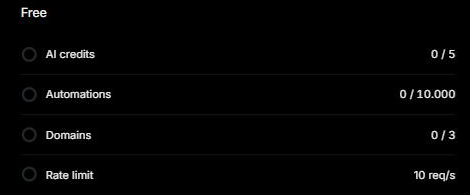
\includegraphics[width=6.4cm]{fig/resend_panel_equipo_2026-09-01.png}};
\node[anchor=south west, font=\scriptsize\bfseries, inner sep=1pt] at (0,0.05) {(a) Observación de panel};
\node[anchor=north west, text width=6.4cm, align=left, font=\scriptsize, inner sep=1pt] at ([yshift=-1mm]img.south west)
  {Panel de una cuenta propia de Resend, plan Free, 1 de septiembre de 2026: el \textit{rate} del equipo es de 10 peticiones por segundo.};
\node[anchor=south west, font=\scriptsize\bfseries, inner sep=1pt] at (8.0,0.05) {(b) Sondeo};
\node[tfm artefacto, text width=24mm, minimum height=13mm, anchor=north west] (pub) at (8.0,-0.15) {\textbf{Lo publicado}\\ \tiny 50 en \texttt{to}; para \texttt{cc} no da tope};
\node[tfm actividad, text width=24mm, minimum height=13mm, anchor=north west] (son) at (11.3,-0.15) {\textbf{Tres peticiones}\\ \tiny contra la API real};
\draw[-stealth] (pub) -- (son);
\node[anchor=north west, inner sep=1pt, font=\tiny] (tab) at (8.0,-1.9) {\scriptsize
  \begin{tabular}{@{}lll@{}}
  \texttt{to} & \texttt{cc} & Respuesta \\ \hline
  51 & 0 & 422, «máximo de 50 en \texttt{to}» \\
  26 & 25 & 422, «no más de 50 en total» \\
  25 & 25 & 200, aceptada \\
  \end{tabular}};
\node[tfm artefacto, text width=58mm, anchor=north west, align=left] (med) at (8.0,-3.45) {\textbf{Lo medido}\\ \tiny el tope de 50 es sobre la suma de \texttt{to} y \texttt{cc}, y la cabecera \texttt{ratelimit-limit}, registrada sin adoptarse, dice 10, como el panel};
\draw[-stealth] (son.south) -- (son.south |- tab.north);
\end{tikzpicture}
\endgroup
